% !TeX root = ../thuthesis-example.tex

\chapter{引言}
\section{研究背景\label{sec:chap1-sec1}}
“物联网”这一术语通常指的是将网络的连接性和计算能力拓展到通常不被视为计算机的物体、传感器和日常物品,使这些设备能够在最小的人工干预下生成、交换和消费数据。物联网这一词汇最早由英国人 Kevin Ashton 在 1999 年用于描述一个系统,在该系统中,物理世界中的对象通过传感器连接到互联网\cite{li2015internet}。一些预测认为,到 2025 年,全球参与物联网的设备数可能达到 1000 亿台,对经济的影响超过 11 万亿美元\cite{rose2015internet}。

在 2013 年德国汉诺威工业展览会上,“工业 4.0”理念首度面世\cite{ghobakhloo2020industry},其中提及的工业物联网(Industrial Internet of Things, IIoT)在全球范围内引起了广泛关注。IIoT 旨在将所有工业资产,包括设备和控制系统,与信息系统和业务流程连接起来。通过收集大量数据,为工业生产、管理和解决方案设计提供重要参考\cite{sisinni2018industrial}。工业物联网会产生大量工业数据,其类型包括时间序列、图片、视频、文档等,在某些场景下一年甚至会产生 $4\times 10^{12}$ GB 数据\cite{ge2012riseofindustrial}。在这些数据中,时间序列数据主要由机器设备上的传感器产生。由于采集频率高、传感器数量多,时序数据成为了工业大数据的主体\cite{di2019industrial}。

工业物联网场景下的时序数据通常具有以下特点:
\begin{enumerate}
  \item 数据产生速度快。例如在风机发电场景下,国际风电标准 IEC 61400-25 规定,每台风机每秒需要采集 225 KB 数据,在某些极端工况下数据的采集频率需要提升至 8 KHz\cite{李天安2020apache}。
  \item 数据总量大。长安汽车集团生产的每一辆汽车上均有数千个传感器,集团的车联网应用一共管理了近 12 亿条时间序列,每年产生的原始数据量超过 13,000 TB。
  \item 数据类型丰富。工业物联网场景下的时序数据除了由传感器产生的整形、长整形、单精度浮点数和双精度浮点数数据外,还可能包括由摄像头产生的图片、视频数据等。
\end{enumerate}

海量的时序数据对数据库的写入、存储和查询都提出了挑战。传统的关系型数据库通常使用 B+ 树作为底层的存储数据结构,其在处理点写入、点查询等负载时具有较好的性能,但是无法满足工业物联网场景下时序数据的批量写入负载和聚合查询负载\cite{jensen2017time}。因此,一种专门为存储时序数据而设计的数据库应运而生,它们被称为时序数据库(Time Series Database,TSDB)。如图 \ref{fig:db-engine} 所示,在国际权威数据库流行度排行机构 DB-Engines 的调查结果中,时序数据库在过去十年内的流行度持续上升,目前其流行度仅次于图数据库,位居榜单中的第二名。

\begin{figure}
  \centering
  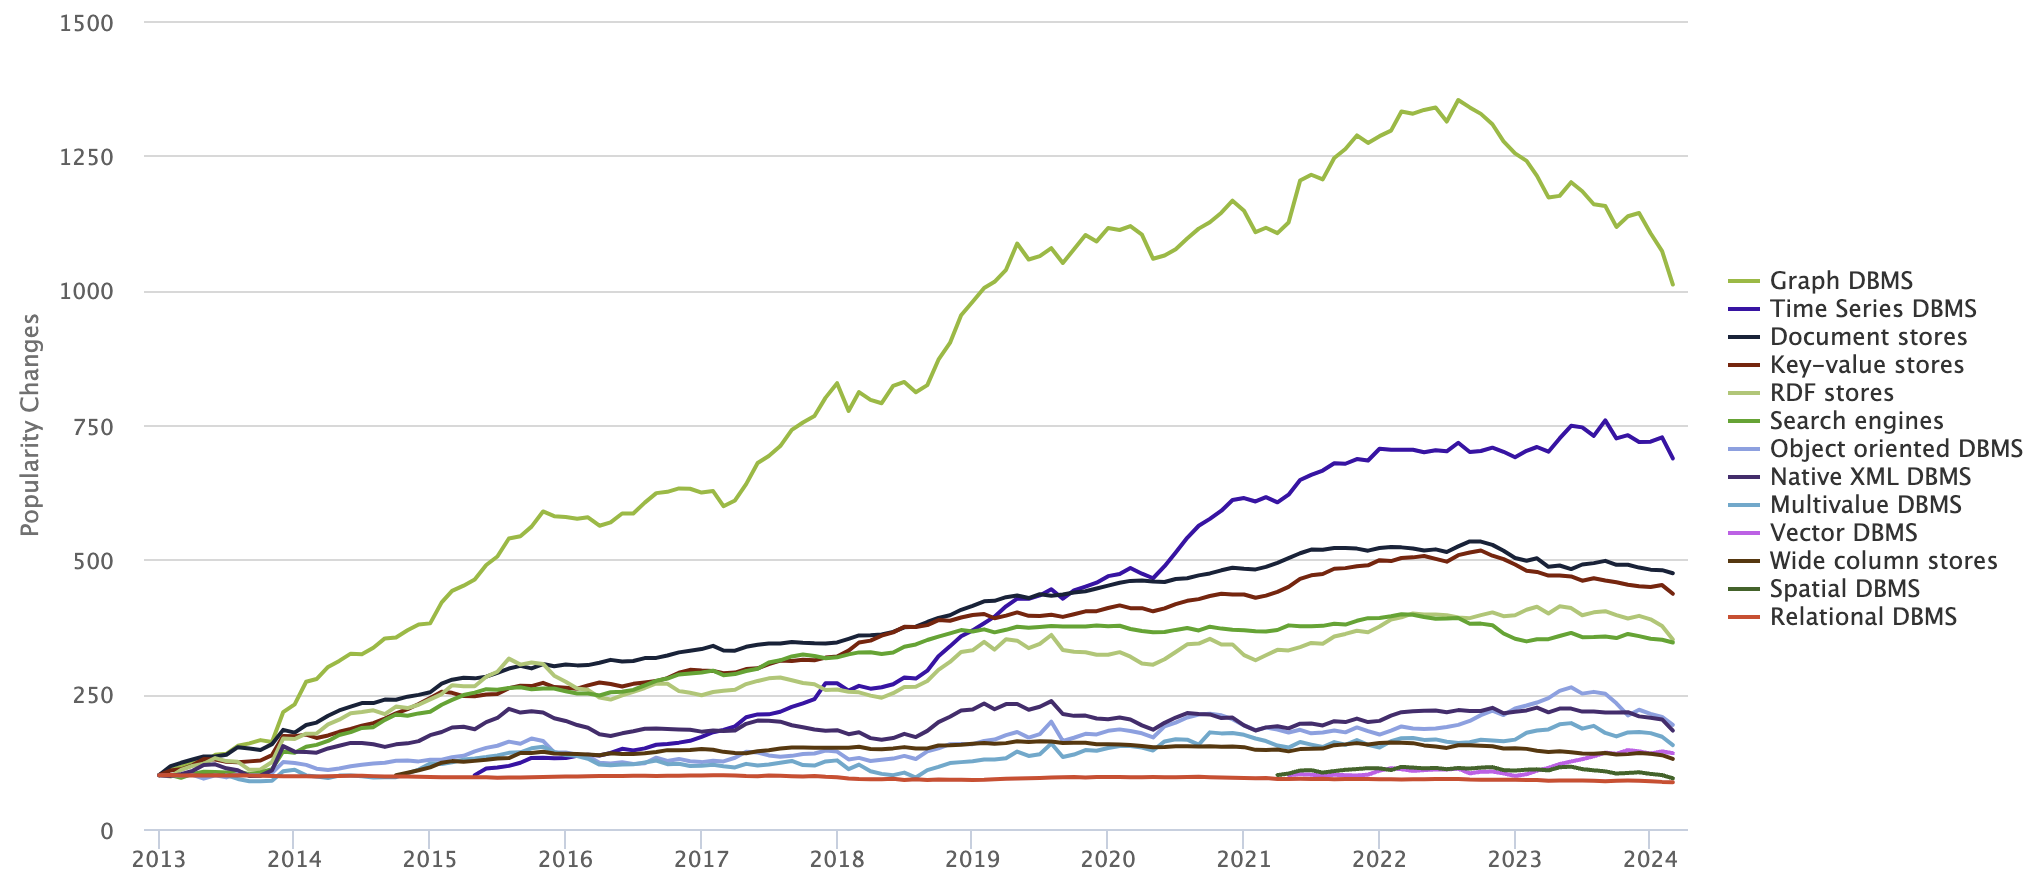
\includegraphics[width=\linewidth]{db-engines-ranking.png}
  \caption{DB-Engines 数据库类型流行度排名}
  \label{fig:db-engine}
\end{figure}

由于时序数据产生速度快、总量大、类型丰富的特点,时序数据库通常对数据的写入机制进行了优化,以满足工业物联网下时序数据的高吞吐写入需求。目前市面上流行的时序数据库主要有 Apache IoTDB\cite{wang2023apache}、InfluxDB\cite{naqvi2017time}、TDEngine\cite{tdengine2024github}、Apache HoraeDB\cite{apache2024horaedb} 等。其中 Apache IoTDB 是 Apache 基金会下一款开源的时序数据库,其具有为时间序列数据所优化的存储引擎、查询引擎以及分布式框架,可以满足工业物联网领域对海量时间序列数据高速写入、存储、快速读取以及复杂查询的需求\cite{wang2020apache}。

Apache IoTDB 使用了常见的客户端-服务器(Client-Server)模式,客户端通过网络向服务器发送写入请求,服务器接收到写入请求后将数据写入到存储引擎中。根据写入请求中数据的内容可以对写入方式进行分类。如果按照一个写入请求中数据所对应的设备数量进行划分,可以将写入方式分为单设备写入和多设备写入。单设备写入指的是一个写入请求中的数据全部来自于一个设备,而多设备写入指的是一个写入请求中的数据可能来自于多个设备。如果按照一个写入请求中数据的数量进行划分,可以将写入方式分为单记录写入和多记录写入。单记录写入指的是一个写入请求中只包含一条记录,而多记录写入指的是一个写入请求中可能包含多条记录。一个单记录写入一定是单设备写入,而一个多记录写入则既可能是单设备写入,也可能是多设备写入。在 IoTDB 被使用的生产场景中,多记录写入是最常见的一种写入方式。

IoTDB 一共提供了三种多记录写入方式:SQL 写入、多 Records 写入(InsertRecords)、单 Tablet 写入(InsertTablet)。其中 SQL 写入和 InsertTablet 都只支持单设备多记录写入,而 InsertRecords 则支持多设备多记录写入。因为多设备多记录写入的灵活性更高,适用的生产场景也更多,因此 InsertRecords 是 IoTDB 使用最广泛的写入方式。但是,目前 IoTDB 的 InsertRecords 写入机制实现不佳,在序列数较多、数据量较大、并发量较高的场景下,这种写入方式无法满足用户的写入需求。提升 InsertRecords 的写入性能有助于满足工业物联网场景下时序数据的高写入负载,降低用户的使用成本,具有重要的现实意义和研究价值。因此,本文的研究重点是如何通过设计和实现上的优化提高 Apache IoTDB 多设备多记录的写入性能。
\section{Apache IoTDB 现有写入机制分析\label{sec:chap1-sec2}}
\subsection{Apache IoTDB 现有多记录写入方式介绍}
如前文所述,Apache IoTDB 目前提供了三种多记录写入方式: SQL 写入、按 Tablet 写入(InsertTablet)、按 Records 写入(InsertRecords)。表 \ref{tab:iotdbwriteinterfacecompare} 对这三种写入方式进行了对比。

SQL 写入指的是使用形如 \emph{insert into root.sg.d1(timestamp, s1, s2) values(1, 1, 2)} 的 SQL 语句进行写入。客户端将 SQL 语句发送到服务器,服务器对 SQL 语句进行解析并生成写入请求,然后将写入请求交由存储引擎处理。这种写入方式较为灵活,大部分时序数据库都会提供这种写入方式。但是,由于每次写入时都需要解析 SQL 语句,这一部分开销不可忽视,因此这种写入方式的性能较差。在生产场景中,几乎没有用户使用这种写入方式。

按 Tablet 写入和按 Records 写入都是 Apache IoTDB 提供的原生数据写入方式,用户将写入请求直接以数据结构的形式传递给客户端,然后客户端通过 RPC 层将这些参数传输到服务器,服务器可以直接从 RPC 层得到写入请求,无需进行 SQL 解析等流程。因此,这两种写入方式的性能远优于通过 SQL 写入的性能。

在 IoTDB 中,一条或多条时间序列归属于同一个设备(Device)\cite{apache2024iotdbdevice}。一个设备对应了现实世界中的一个实体,是一个在现实世界中拥有若干个物理量的装置,例如一台风力发电机、一辆汽车、一台计算机等。每个设备在 IoTDB 中都有唯一的 ID,称为设备 ID。每个设备下的时间序列也有其 ID,称为时间序列 ID。每条时间序列的 ID 和其所属设备的 ID 组成了该时间序列的唯一标识符。

按 Tablet 写入需要用户在代码中将一批数据组织成名为 Tablet 的数据结构,然后通过 IoTDB 的客户端 SDK 发送到服务器。一个 Tablet 是一个设备在一段时间内的多行数据,每一行数据都有不同的时间戳。按 Tablet 写入的本质是在时间维度上将同一个设备的数据聚集起来批量写入到 IoTDB 中,不同设备的数据无法聚集在同一个 Tablet 中。多记录写入的好处是可以将写入流程中的某些代价(例如元数据校验的代价、执行流程中的锁获取的代价等)均摊到多条数据上,进而提升写入的性能。因此,如果想要获得较好的写入性能,写入的单个 Tablet 数据量不能太少,否则就失去了多记录写入的优势。

按 Tablet 写入的方式非常适合单设备数据高频产生的场景,因为单个设备数据产生的频率快,在较短时间内就可以构建一个合适大小的 Tablet 进行写入,数据从产生到写入数据库的间隔较短。但是在单设备数据低频产生的场景下,如果使用按 Tablet 写入,就需要较长时间才能构建一个合适大小的 Tablet,数据从产生到写入数据库的间隔会大大增加。例如在长安汽车集团的车联网场景中,一辆汽车被建模为一个设备,汽车中的每个传感器(如胎压、水温等)则是设备下的时间序列。每辆汽车每 30 秒采集一次车内传感器的数据,如果按照一个 Tablet 有 100 行数据计算,那么每辆汽车的数据从产生到写入数据库的间隔会达到 50 分钟,而在这期间用户无法查询到这些数据,这显然是无法接受的。

按 Records 写入是多记录写入的另一种形式。一条 Record 是一个设备在一个时间戳下产生的一行数据,Records 是多个 Record 的组合,可能包含多个设备在多个时间戳下的数据。这种写入方式本质上是在时间和设备两个维度上将数据聚集在一起进行批量写入。这种写入方式避免了按 Tablet 写入的缺点,即使单个设备产生数据的频率较低,也可以将多个低频设备的数据组合起来进行批量写入。这样既通过多记录写入提升了写入性能,又避免了数据从产生到写入数据库间隔过长的问题。因此,按 Records 写入是 IoTDB 目前适用场景最广的写入方式。但是,由于过去设计和实现不佳,在单设备数据高频写入等场景下按 Records 写入的性能与按 Tablet 写入的性能有一定差距,因此如何优化按 Records 写入的设计和实现进而提升其性能是本文关注的重点。

\begin{table}
  \centering
  \caption{Apache IoTDB 写入方式对比}
  \begin{tabular}{lp{3.5cm}p{3.5cm}p{3.5cm}}
    \toprule
    写入接口  & 优点 & 缺点 & 适用场景 \\
    \midrule
    SQL 写入 & 灵活 & 性能较差 & 用户测试或少量数据写入 \\
    按 Tablet 写入  & 性能最好,可以将写入流程中的某些固定开销均摊到一批数据上 & 单设备数据低频产生的场景下,数据从产生到真正写入的延迟较大 & 单设备数据高频产生的场景\\
    按 Records 写入  & 性能较好,即可以通过多记录写入获取不错的性能,又降低了数据从产生到真正写入的延迟 & 由于设计和实现原因,性能与按 Tablet 写入有差距 & 单设备数据低频或高频产生的场景 \\
    \bottomrule
  \end{tabular}
  \label{tab:iotdbwriteinterfacecompare}
\end{table}

\subsection{Apache IoTDB 现有按 Records 写入机制实现}
如图\ref{fig:iotdb-write-process}所示,目前 IoTDB 按 Records 写入流程主要分为三个阶段:
\begin{enumerate}
  \item 客户端 SDK 进行数据预处理。此阶段从 IoTDB 客户端的写入 SDK 被用户调用开始,到客户端调用远程过程调用层的数据发送方法前结束。这个阶段进行的工作是检验用户传入的参数是否合法,检查客户端状态,选取合适的服务器节点作为数据发送的目标(因为在分布式部署时 IoTDB 可能存在多个服务器节点),对待写入数据进行部分序列化。
  \item 远程过程调用层进行数据传输。远程过程调用(Remote Procedure Call,RPC)层连接了客户端和服务器,其负责的主要工作为:将客户端传入的数据根据预定义的结构序列化为二进制的数据流,并通过网络传输到服务器,再反序列化为预定义的数据结构,交由服务器中 IoTDB 上层的写入逻辑进行处理。
  \item IoTDB 服务器处理写入请求。此时写入请求被 RPC 层反序列化为预定义的写入请求数据结构,IoTDB 会进行时间序列 ID 检查、元数据检查、权限检查、MPP 框架处理、内存控制处理、监控框架记录性能指标、写预写日志(Write Ahead Log,WAL)、写入内存表、更新内存索引等步骤,最终将数据记录在内存和磁盘中。这一步结束以后,整个写入请求就执行成功了。
\end{enumerate}
\begin{figure}
  \centering
  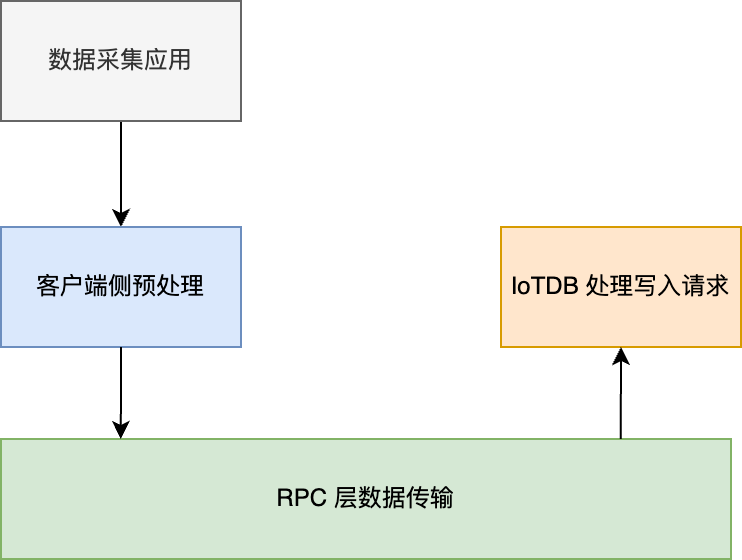
\includegraphics[width=0.55\linewidth]{数据写入整体过程.png}
  \caption{Apache IoTDB 数据写入流程}
  \label{fig:iotdb-write-process}
\end{figure}
\subsection{Apache IoTDB 现有多设备多记录写入机制不足}
经过在某些用户场景和压力测试场景下对 Apache IoTDB 的 InsertRecords 写入机制的测试和分析,本工作发现其有以下问题:
\begin{enumerate}
  \item 服务器写入存储引擎的过程实现得不够高效。当一批记录一起到达 IoTDB 的服务器 后,目前写入存储引擎时仍然是逐条进行写入,而不是批量化地写入。这样的实现方式需要在写入每一行记录时都获取写入路径上的多个锁,在监控框架中更新指标,调用很多预处理和后处理函数。这些操作都会带来很大的开销,使得服务器上真正用于记录数据的时间比例较低,资源利用比较低效。
  \item 写入请求序列化过程较低效。目前 IoTDB 所使用的 RPC 框架是 Apache Thrift,然而目前 InsertRecords 写入机制的实现直接将客户端传入的参数放到了 Thrift 中进行传输。而 Thrift 的序列化方案设计初衷是为了保持较高的兼容性,对于时序数据的写入则没有进行优化。这样的序列化方式会导致序列化和反序列化的开销较大,影响了写入性能。
  \item 对客户端侧的资源利用不足。目前 IoTDB 的客户端侧所执行的工作较为轻量,部分与上下文无关的工作,如路径语法校验、内存占用计算等工作都在服务器侧进行,这并没有充分利用客户端侧的资源,也没有充分利用客户端侧的计算能力。
\end{enumerate}
由于篇幅原因,对原有多设备多记录写入机制不足的详细分析将在后续章节中进一步展开。
\section{研究内容}
结合 \ref{sec:chap1-sec1} 和 \ref{sec:chap1-sec2} 节的分析,本文发现目前 Apache IoTDB 的多设备多记录写入方式具有较高的灵活性,但是过去的实现机制在性能上存在一定的不足,在时间序列数较多、写入数据量较大的场景下无法很好地满足用户需求。因此,本工作的研究内容主要包括:
\begin{enumerate}
  \item 分析目前多设备多记录写入性能较差的原因。目前 IoTDB 的多设备多记录写入方式的性能与单设备多记录写入方式的性能大约有 2-3 倍的差距,分析这个差距产生的原因有助于可以指导后续对多设备多记录写入机制的优化。
  \item 在保持目前客户端多设备多记录写入 SDK 不变的情况下对写入性能进行优化。由于目前使用 Apache IoTDB 多设备多记录写入方式的用户较多,因此优化多设备多记录写入的性能时需要保持对原有代码的兼容,避免为用户带来较高的迁移成本。同时,优化后的多设备多记录写入性能应该有较大提升,以满足用户的写入需求。
  \item 对优化措施进行合理的评估。在优化多设备多记录的写入性能后,需要对优化措施进行性能评估与分析,以验证优化效果。目前的性能测试工具并不能很好地反映用户的真实写入场景,因此本工作需要开发一套模拟用户场景的测试工具,收集真实用户场景的写入特征,并使用测试工具根据这些特征模拟不同用户的写入场景,验证并分析优化措施的有效性。
\end{enumerate}

\section{研究贡献}
本文的主要贡献体现在以下三个方面:
\begin{enumerate}
  \item \textbf{对目前 Apache IoTDB 已有多设备多记录写入机制的性能分析}。本工作对目前 Apache IoTDB 的已有多设备多记录写入机制进行了性能分析,找出了其性能瓶颈,并指出了其在设计上和实现上的不足之处。
  \item \textbf{对 Apache IoTDB 多设备多记录写入机制进行优化}。基于本工作对已有多设备多记录写入机制分析出的缺陷,分别从客户端、RPC 层、存储引擎侧进行优化,提高了多设备多记录写入的性能。
  \item \textbf{对 Apache IoTDB 的多设备多记录写入机制优化措施的性能评估与分析}。本工作开发了一套模拟用户场景的测试工具,收集了一些真实用户场景的写入特征,并使用测试工具根据这些特征模拟不同用户的写入场景,验证并分析优化措施的有效性。
\end{enumerate}

\section{本文的组织结构}

本文一共分为八章,每个章节的内容如下:

第 1 章为引言部分,主要介绍了物联网和工业物联网发展背景下时序数据库发展的意义,并介绍了目前 Apache IoTDB 的三种写入方式及其优缺点和适用场景,并阐述了目前 Apache IoTDB 多设备多记录写入的不足之处,最后引出了本工作的研究内容和贡献。

第 2 章介绍了相关工作,首先介绍了主流时序数据库的写入方式,然后介绍了和客户端优化相关的研究。

第 3 章详细介绍了目前 Apache IoTDB 的多设备多记录写入机制的运行流程,包括客户端侧的数据预处理、RPC 层的数据传输、服务器端的写入处理等,并通过 Arthas 等工具对这一机制的性能进行了分析,找出了其性能瓶颈,并指出导致瓶颈出现的原因。随后从整体上介绍了本工作的优化目标和优化思路,包括对客户端、RPC 层、存储引擎的优化,为读者对本工作提供一个整体的认识。

第 4 章介绍了对客户端侧的设计和实现,包括对客户端侧的数据预处理、写入请求格式转换、路径校验、内存开销预计算等方面的设计与实现,并介绍了实现过程中的一些细节。

第 5 章介绍了对多设备多记录写入请求序列化的优化,介绍了基于信息类型的序列化方案,包括对元数据区、数据区以及辅助数据区的序列化设计与实现。

第 6 章介绍了对服务器侧多设备多记录写入机制的优化措施,包括批量化写入、计划片级并行写入、预写日志压缩等。

第 7 章是实验部分,首先介绍了用于模拟用户场景的测试程序的设计,然后介绍了包括中冶赛迪、长安汽车、四维智联等用户的典型写入场景,最后使用模拟测试工具和 IoT-Benchmark\cite{liu2019benchmarking} 两种测试工具对优化后的多设备多记录写入机制进行了性能测试,并对测试结果进行了分析。

第 8 章是总结部分,总结了本文的工作,指出了本文的不足之处,并对未来的工作进行了展望。